% !TEX root = ../../技术文档.tex
\section{FPGA实现}

FPGA顶层集成TriHaRiscv SoC、视频子系统、共享DDR互连及板级支撑逻辑，整体结构如图\ref{fig:fpga-top-modules}所示。
SoC与Video作为两个独立模块，通过寄存器接口传递采集和显示控制信息，通过共享DDR交换帧数据、模型输入及计算结果。
HDMI收发芯片、DDR3芯片和USB-UART接口位于FPGA之外，由顶层完成信号连接与时序适配。

\begin{figure}[!htbp]
\centering
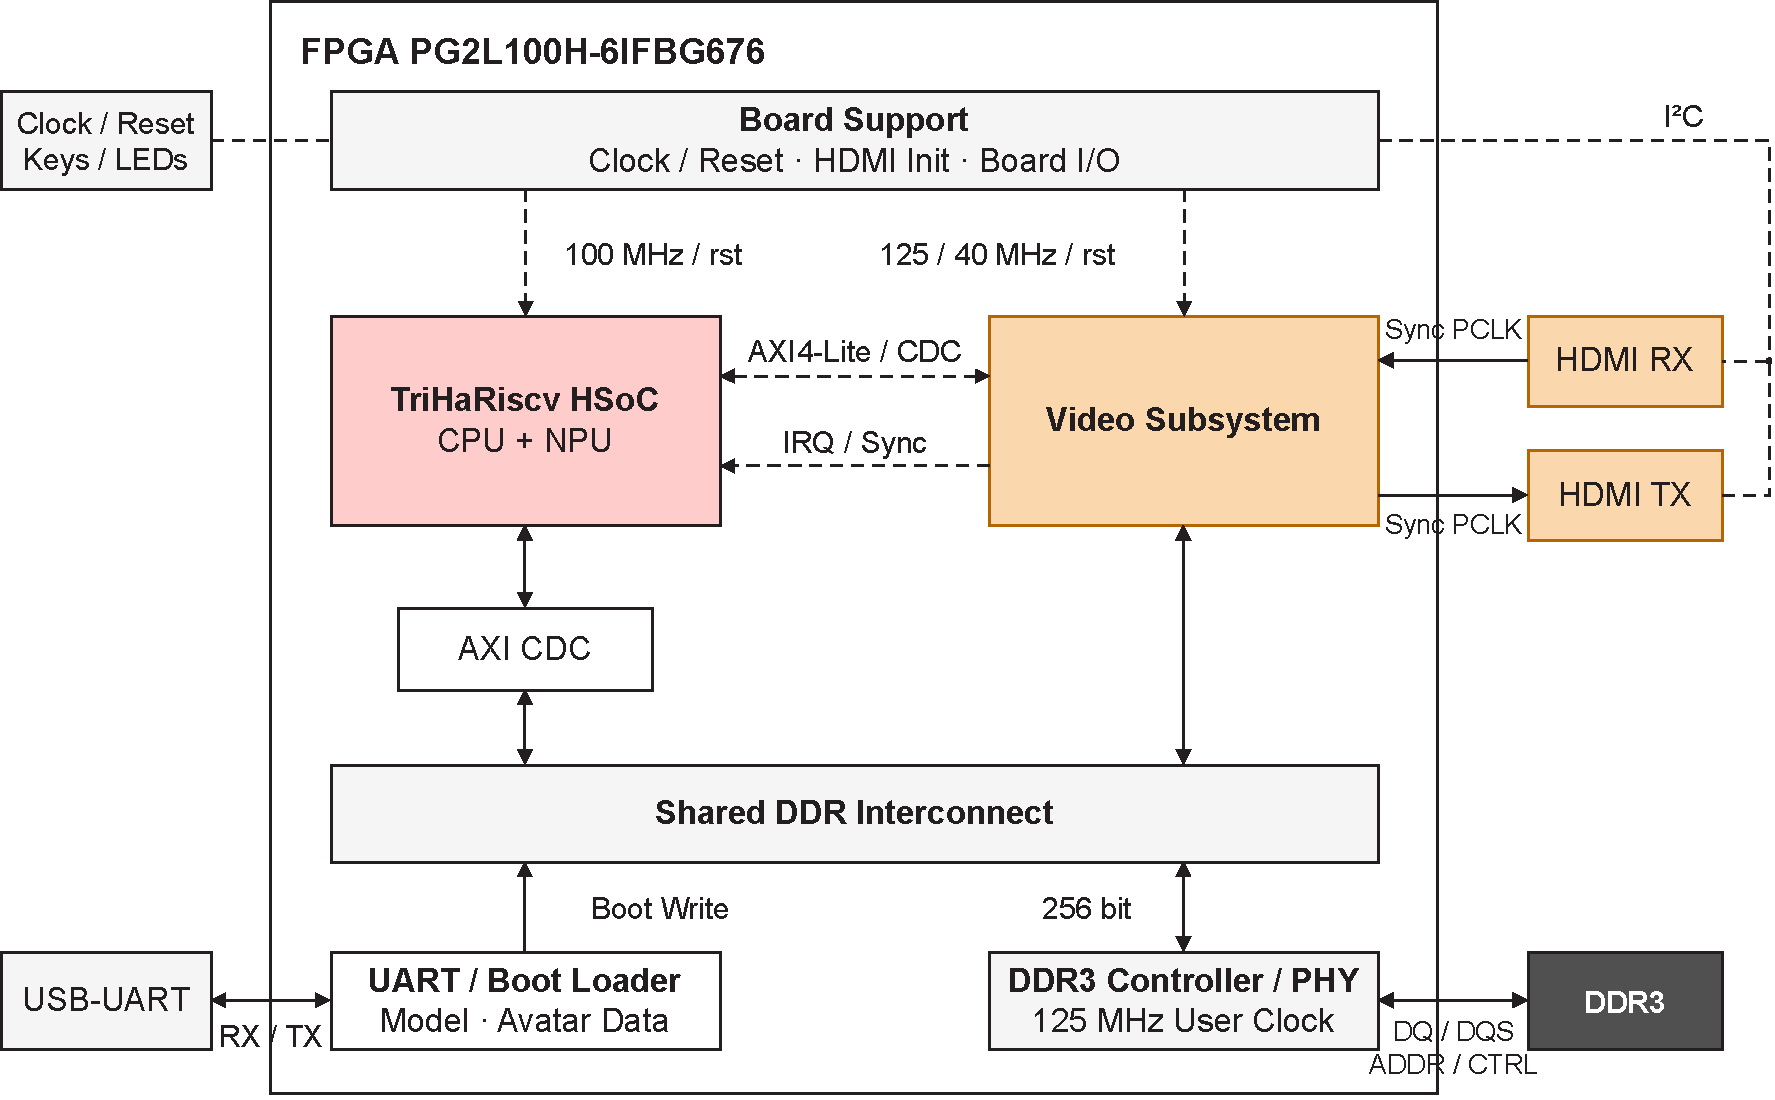
\includegraphics[width=\linewidth]{../figure/fpga-top.pdf}
\caption{FPGA顶层架构与板级接口}\label{fig:fpga-top-modules}
\end{figure}

SoC内部包含CPU、NPU、片上存储和控制接口，人脸检测应用运行于50\,MHz计算时钟域。
CPU与NPU的外存事务汇入128\,bit AXI4通路，经跨时钟域桥进入125\,MHz的共享DDR互连。
Video的采集写入和显示读取直接接入该互连；其控制寄存器通过AXI4-Lite跨域桥与SoC连接，中断信号经同步后送入SoC。
共享互连完成访问仲裁及128\,bit至256\,bit的位宽转换，通过厂商IP用户端口连接DDR3控制器与PHY，再由32\,bit物理接口访问板载DDR3。

串口装载器在启动阶段接收模型程序、参数、CPU解码表、三份输出头初值及RGBA头像，经共享DDR写通路写入约定地址。
七段数据通过写入确认与CRC校验并封存后，启动写通路交还给视频采集逻辑，头像读取器从DDR校验并填充片上缓存。运行期间的采集、推理与显示共同使用同一DDR控制器。
HDMI接收芯片提供RGB像素、同步信号和输入像素时钟；视频子系统完成采集、预处理与显示合成后，将输出像素和同步信号送入HDMI发送芯片。

板级支撑逻辑集中处理时钟分配、复位同步、HDMI芯片初始化及按键和LED接口。
计算时钟和输出像素时钟由PLL生成，125\,MHz的Video核心与DDR用户时钟由DDR IP提供，各时钟域分别同步释放复位。
HDMI收发芯片通过I\textsuperscript{2}C完成初始化，输入像素跨域采用异步FIFO。
图中实线表示数据连接，虚线表示控制、时钟及复位关系。

\subsection{目标平台}

本设计采用盘古100pro+开发板，主控为紫光同创Logos-2系列PG2L100H-6IFBG676。
CPU、NPU和视频逻辑使用片上LUT、FF、APM及DRM实现，器件资源容量依据Logos2数据手册，平台主要配置见表\ref{tbl:platform}。
板载DDR3由两颗4\,Gbit芯片组成，总容量1\,GB，数据通路32\,bit；
模型程序、参数、中间张量和三帧槽位于软件规划的DDR窗口中。

\begin{reporttable}
\footnotesize
\begin{longtable}{@{}lll@{}}
\caption{平台配置表}\label{tbl:platform}\\
\toprule
项目 & 配置 & 说明或用途 \\
\midrule
\endfirsthead
\caption[]{平台配置表（续）}\\
\toprule
项目 & 配置 & 说明或用途 \\
\midrule
\endhead
\bottomrule
\endfoot
开发板 & 盘古100pro+（MES2L676-100HP） & FPGA及板级外设平台 \\
主控器件 & PG2L100H-6IFBG676 & 紫光同创Logos-2系列FPGA \\
逻辑资源 & 66,600个LUT，133,200个FF & CPU、NPU及系统控制逻辑 \\
运算资源 & 240个APM & 乘法与MAC运算 \\
片上存储 & 155个36Kbit DRM & CPU存储、Cache及NPU缓冲区 \\
外部存储 & 1GB DDR3，2颗4Gbit芯片，32bit数据位宽 & 模型参数、特征图及视频帧存储 \\
视频接口 & 1路HDMI输入、1路HDMI输出 & 视频接入与显示 \\
通信接口 & USB-UART & 板载通信与串口调试 \\
辅助接口 & 按键、LED、SD卡接口 & 控制输入、状态显示及扩展存储 \\
下载与供电 & JTAG、12V电源接口 & 比特流下载、逻辑调试和板卡供电 \\
\end{longtable}
\end{reporttable}

开发板实物及连接如图\ref{fig:board-photo}所示。
图中可见FPGA核心板、板载DDR3及HDMI输入输出接口，外接JTAG下载器用于比特流下载与逻辑调试。

\begin{figure}[!htbp]
\centering
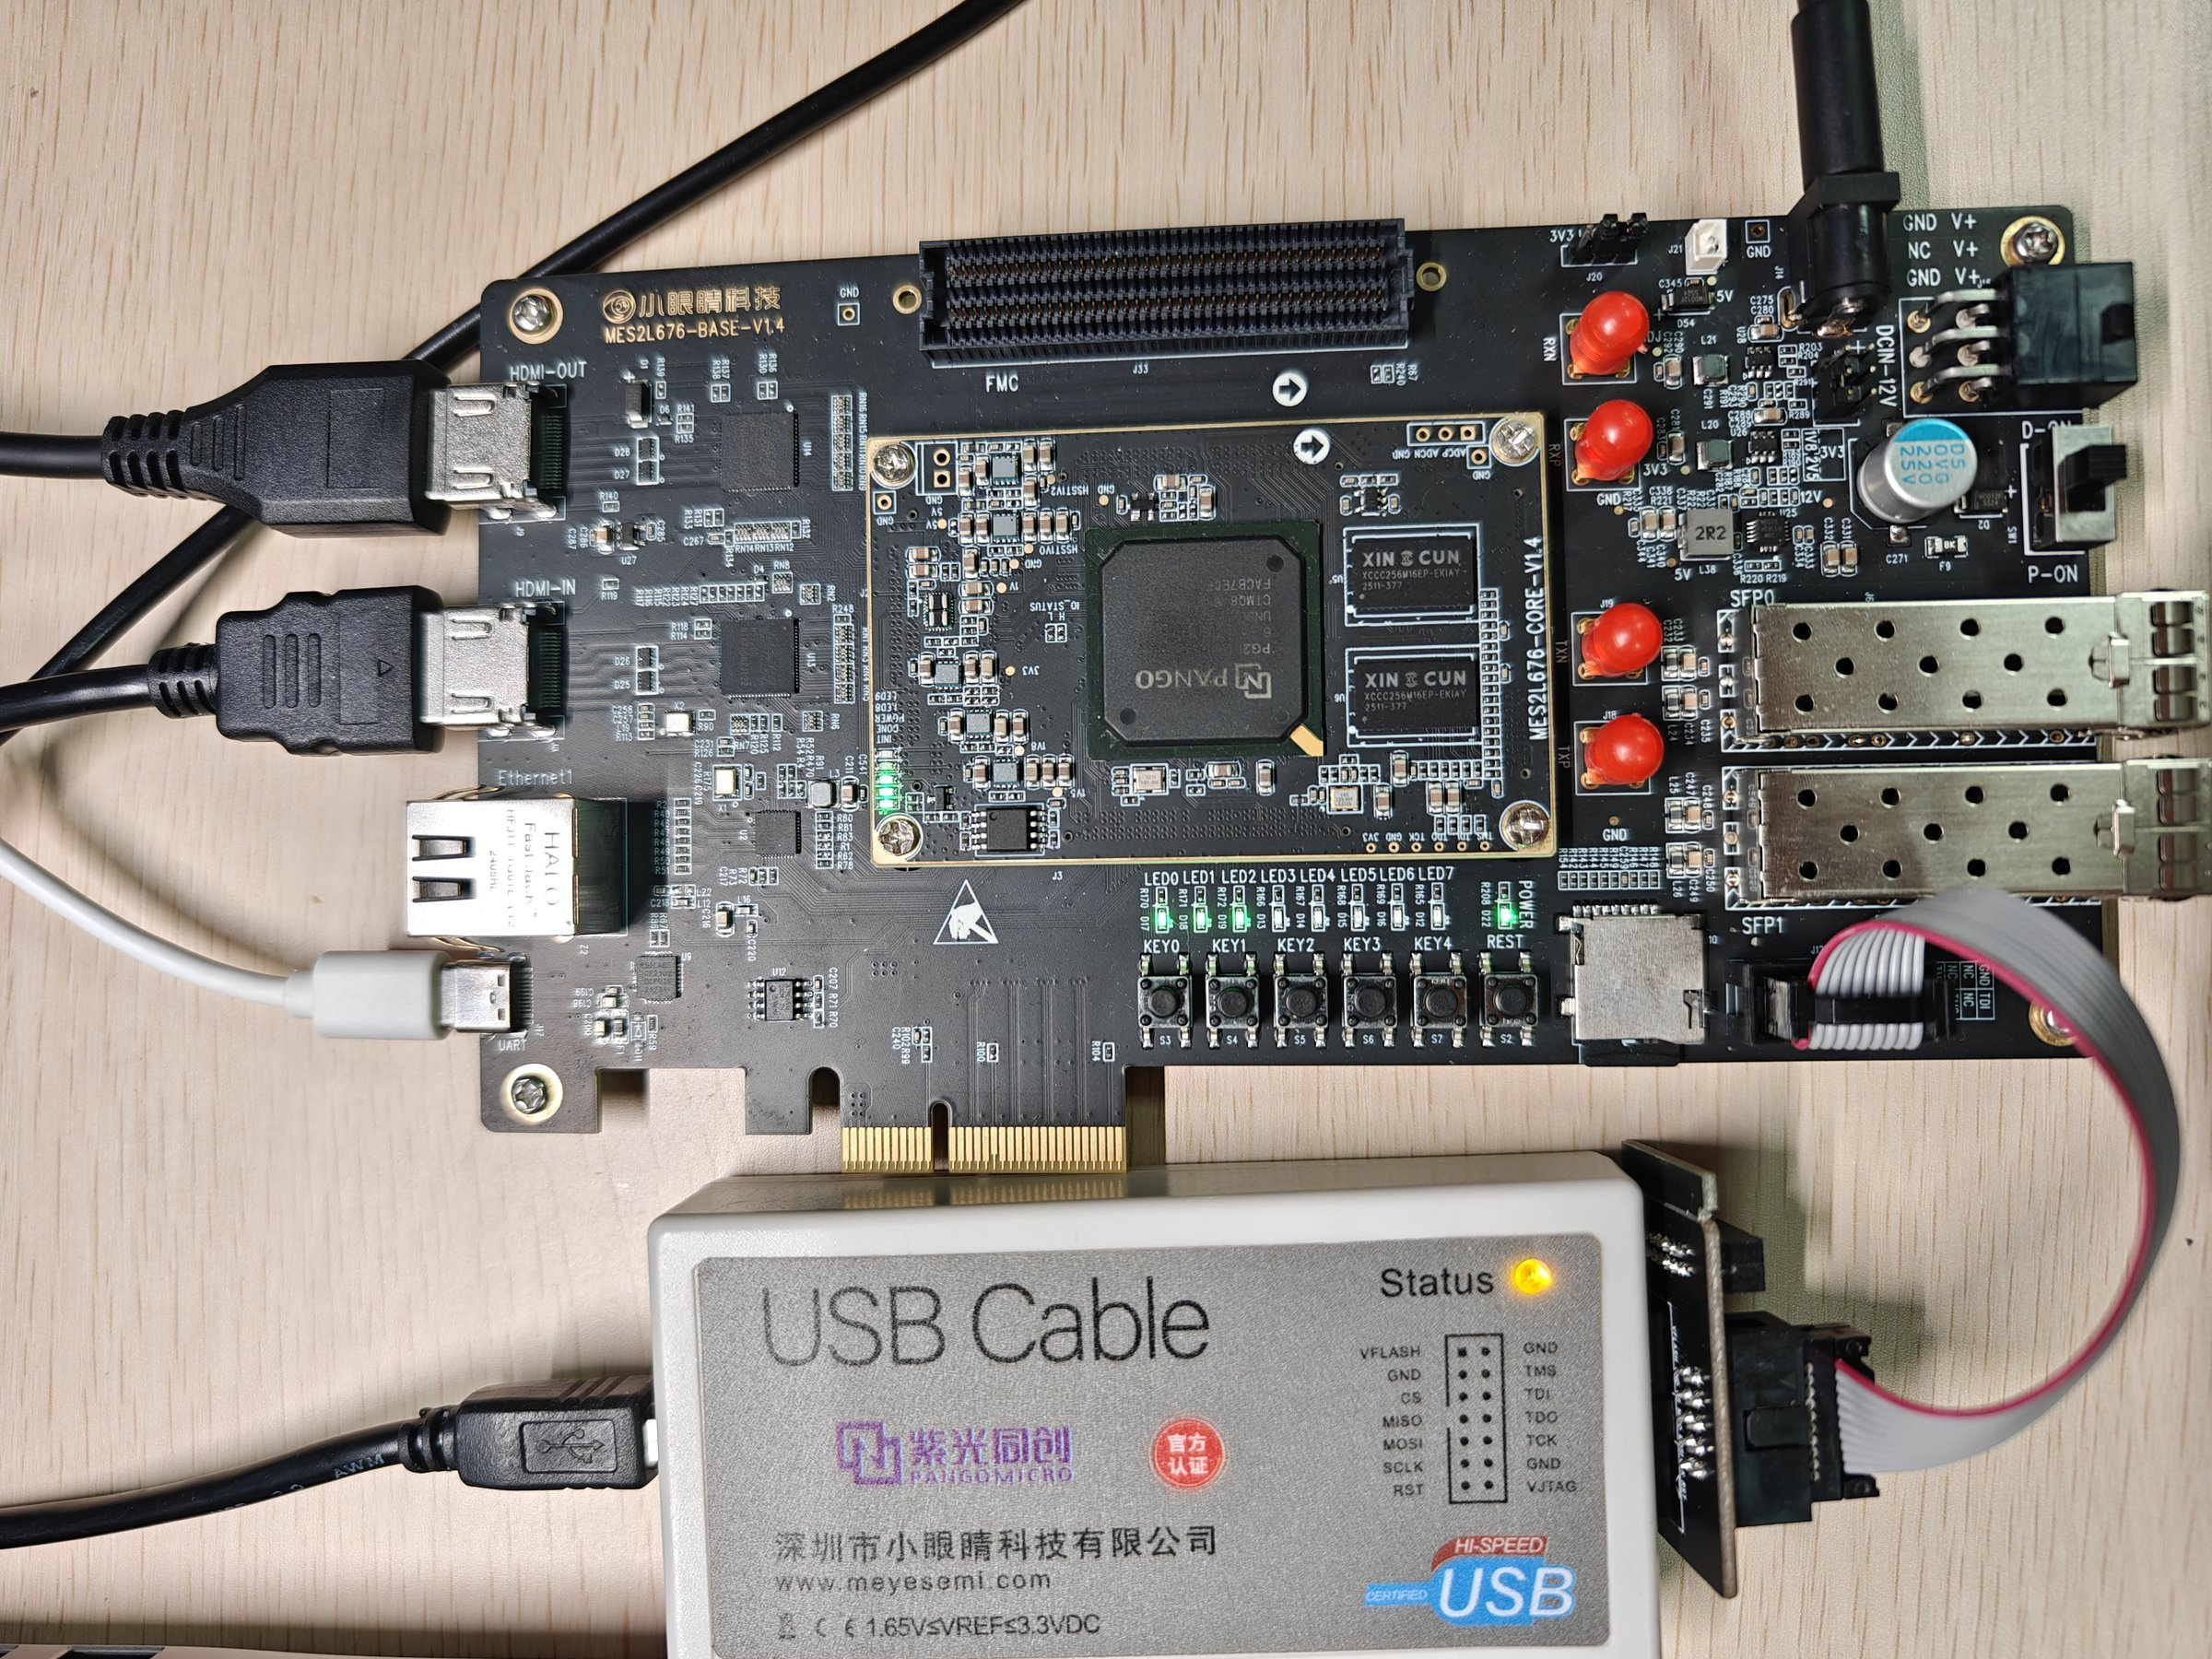
\includegraphics[width=0.69\linewidth]{../figure/pangu100pro-board-photo.jpg}
\caption{盘古100pro+开发板实物}\label{fig:board-photo}
\end{figure}

\subsection{资源统计}

表\ref{tbl:board-resources}列出人脸检测整机的综合资源，统计对象为同一综合网表中的顶层及主要模块层级。
DRM按36\,Kbit等效块计，两个18\,Kbit原语计为一个等效块；LUT总数包含分布式RAM。
整机采用单发射控制CPU、两空间行Dense阵列、单量化通路和RAW、BOX、AVATAR显示配置，包含固定照片的无损行区间缓存及合成流水。

\begin{reporttable}
\small
\begin{longtable}{@{}p{0.43\linewidth}rrrr@{}}
\caption{人脸检测整机综合资源}\label{tbl:board-resources}\\
\toprule
统计对象 & LUT & FF & DRM & APM \\
\midrule
\endfirsthead
\caption[]{人脸检测整机综合资源（续）}\\
\toprule
统计对象 & LUT & FF & DRM & APM \\
\midrule
\endhead
\bottomrule
\endfoot
整机顶层 & 45716 & 41848 & 113.5 & 64 \\
应用CPU及本地存储、路由 & 3416 & 2739 & 18.5 & 4 \\
NPU & 22968 & 17818 & 33.5 & 49 \\
Video应用引擎 & 9944 & 11920 & 43.5 & 10 \\
DDR厂商IP & 4701 & 5157 & 0 & 0 \\
共享DDR仲裁与桥接 & 1350 & 689 & 4 & 0 \\
计算数据跨域桥 & 71 & 153 & 7 & 0 \\
视频控制跨域桥 & 61 & 149 & 2.5 & 0 \\
\end{longtable}
\end{reporttable}

顶层占用器件68.64\%的LUT、31.42\%的FF、73.23\%的DRM和26.67\%的APM。
模块行均包含在整机总数中；顶层还包括装载、初始化及状态控制逻辑，合计直接采用顶层报告。
应用CPU一行包含ROM、SRAM和地址路由，与第三部分独立CoreMark测试中的CPU核统计范围分别记录。

NPU的A、B和O缓冲声明容量各为16\,KiB，ROI为64\,KiB，行暂存为4\,KiB；部分和保存在计算通路的累加器中。
综合依据空间并行度和有效端口裁剪存储体，表中33.5个DRM等效块为该配置的实际映射结果。
资源、后布线及配置校验记录保存于\path{docs/verification/soc/face_photo_report_20261104/}。

\subsection{工程配置}

工程以SoC、CPU、NPU和Video独立验证顶层共用一份RTL，板级目录集中管理DDR、HDMI、PLL、引脚和时序约束。
CPU发射宽度、Cache与分支预测开关、NPU并行度、地址映射及视频模式在综合前确定。
人脸检测顶层采用单发射精简控制CPU，应用代码和数据位于片上SRAM；NPU空间并行度为2，量化通路数为1，图控制器执行完整模型，CPU完成九头输出的后处理。
视频配置采集原图与模型输入，显示端按模式输出原图、全部有效检测框或主人脸位置的透明头像。CPU独立验证顶层另通过\texttt{DUAL\_ISSUE}和\texttt{CACHE\_ENABLE}配置发射宽度与缓存。
构建流程依次生成存储初始化文件、综合网表、布局布线结果和位流。

发布包记录源码提交、工具与IP版本、硬件配置、固件及模型哈希。
软件装载地址与链接布局相互核对，位流、固件和数据包按同一接口版本配套使用。

\subsection{时钟复位}

CPU、NPU和SoC控制逻辑使用独立PLL产生的50\,MHz计算时钟；Video预处理、DMA及本地存储控制使用125\,MHz核心时钟。
计算PLL以125\,MHz参考时钟为输入，生成时钟约束采用$2/5$频率比，与实际PLL输出一致。
HDMI输入使用接收侧像素时钟，输出使用40\,MHz像素时钟；DDR用户时钟按厂商IP配置。
相关异步输入分别同步，像素数据跨域使用异步FIFO，多位地址、帧标识和显示记录使用保持数据束及握手\cite{cummings2008cdc}。

复位在各本地域同步释放。CPU可先从ROM/SRAM启动，DDR初始化成功后才开放外存DMA，
视频输出先产生本地背景，再接受完整有效帧。失锁和整机重初始化同时处理旧事务、FIFO与帧所有权。

\subsection{板级接口}

HDMI一入一出均采用800$\times$600固定模式，接收和发送芯片通过板级控制接口完成初始化。
DDR3接口连接板载32\,bit存储通路，USB-UART承担模型、头像装载及确认响应，接口使用115200波特率、8位数据、无校验和1位停止位。
KEY0（C22）提供协调复位，KEY1（C23）经同步和20\,ms消抖后请求循环切换显示模式，LED指示运行状态，JTAG用于FPGA配置和逻辑调试。

板级封装根据原理图定义引脚方向、电平和I/O标准，输入输出像素与同步信号保持对应时序。
应用固件随片上存储初始化内容配置，模型程序、权重参数、解码表、输出头初值和头像通过串口写入约定地址，封存后由FPGA执行处理和显示。

\subsection{实现约束}

内部时序约束覆盖计算、DDR用户、输入像素和输出像素时钟，并定义PLL生成关系及复位同步路径。
跨域例外对应具体FIFO或握手结构，数据总线与控制信号按其同步方式设置约束。
布局布线后分别分析各时钟域的建立保持裕量、关键路径和跨域结构。

后布线检查包含建立、保持、恢复、移除及最小脉宽，并对异步FIFO的Gray指针数据路径和源、目的时钟偏差进行核对。
本配置的内部时序及CDC检查通过，双角结果在第三部分汇总；实际工作频率按相应时钟约束列出。
最差建立路径位于125\,MHz DDR用户时钟域内的模型输入采集DMA控制逻辑，其寄存器起止点、逻辑级数及延迟构成见表\ref{tbl:board-critical-setup}。
内部STA核对已约束的寄存器路径，CDC核对异步FIFO与握手结构的数据及控制时序；DDR初始化、模型装载和HDMI画面观察属于板级功能验收。
外部DDR PHY与HDMI I/O的板级AC约束和裕量需单独验收，内部正裕量不能替代这项检查。
